	\chapter{行人导航系统设计与实现}
	
	\section{系统设计目标与需求}
	
	本行人导航系统设计目标是在复杂城市环境中为行人提供有效导航支持,利用智能技术引导避开障碍物并高效到达目的地,为此系统须具备以下核心功能:根据用户提供的起点和终点坐标,实时计算最优路径,综合考虑最短距离、行人行走速度、道路状况及交通规则等因素;具备实时障碍物检测与避让功能,及时识别并避开动态环境中的障碍物如其他行人、交通事故、施工区域等;持续监控周围环境并动态调整行进路线,应对突发障碍物或路线变化;具备极高实时响应能力,迅速感知环境变化并及时做出路径调整与决策。系统设计需在复杂动态环境中提供快速、精确、安全的行人导航服务。在这个系统中,设置的目标地点和起始地点如图 \ref{fig:location}所示:
	
	\begin{figure}[H]
	    \centering
	    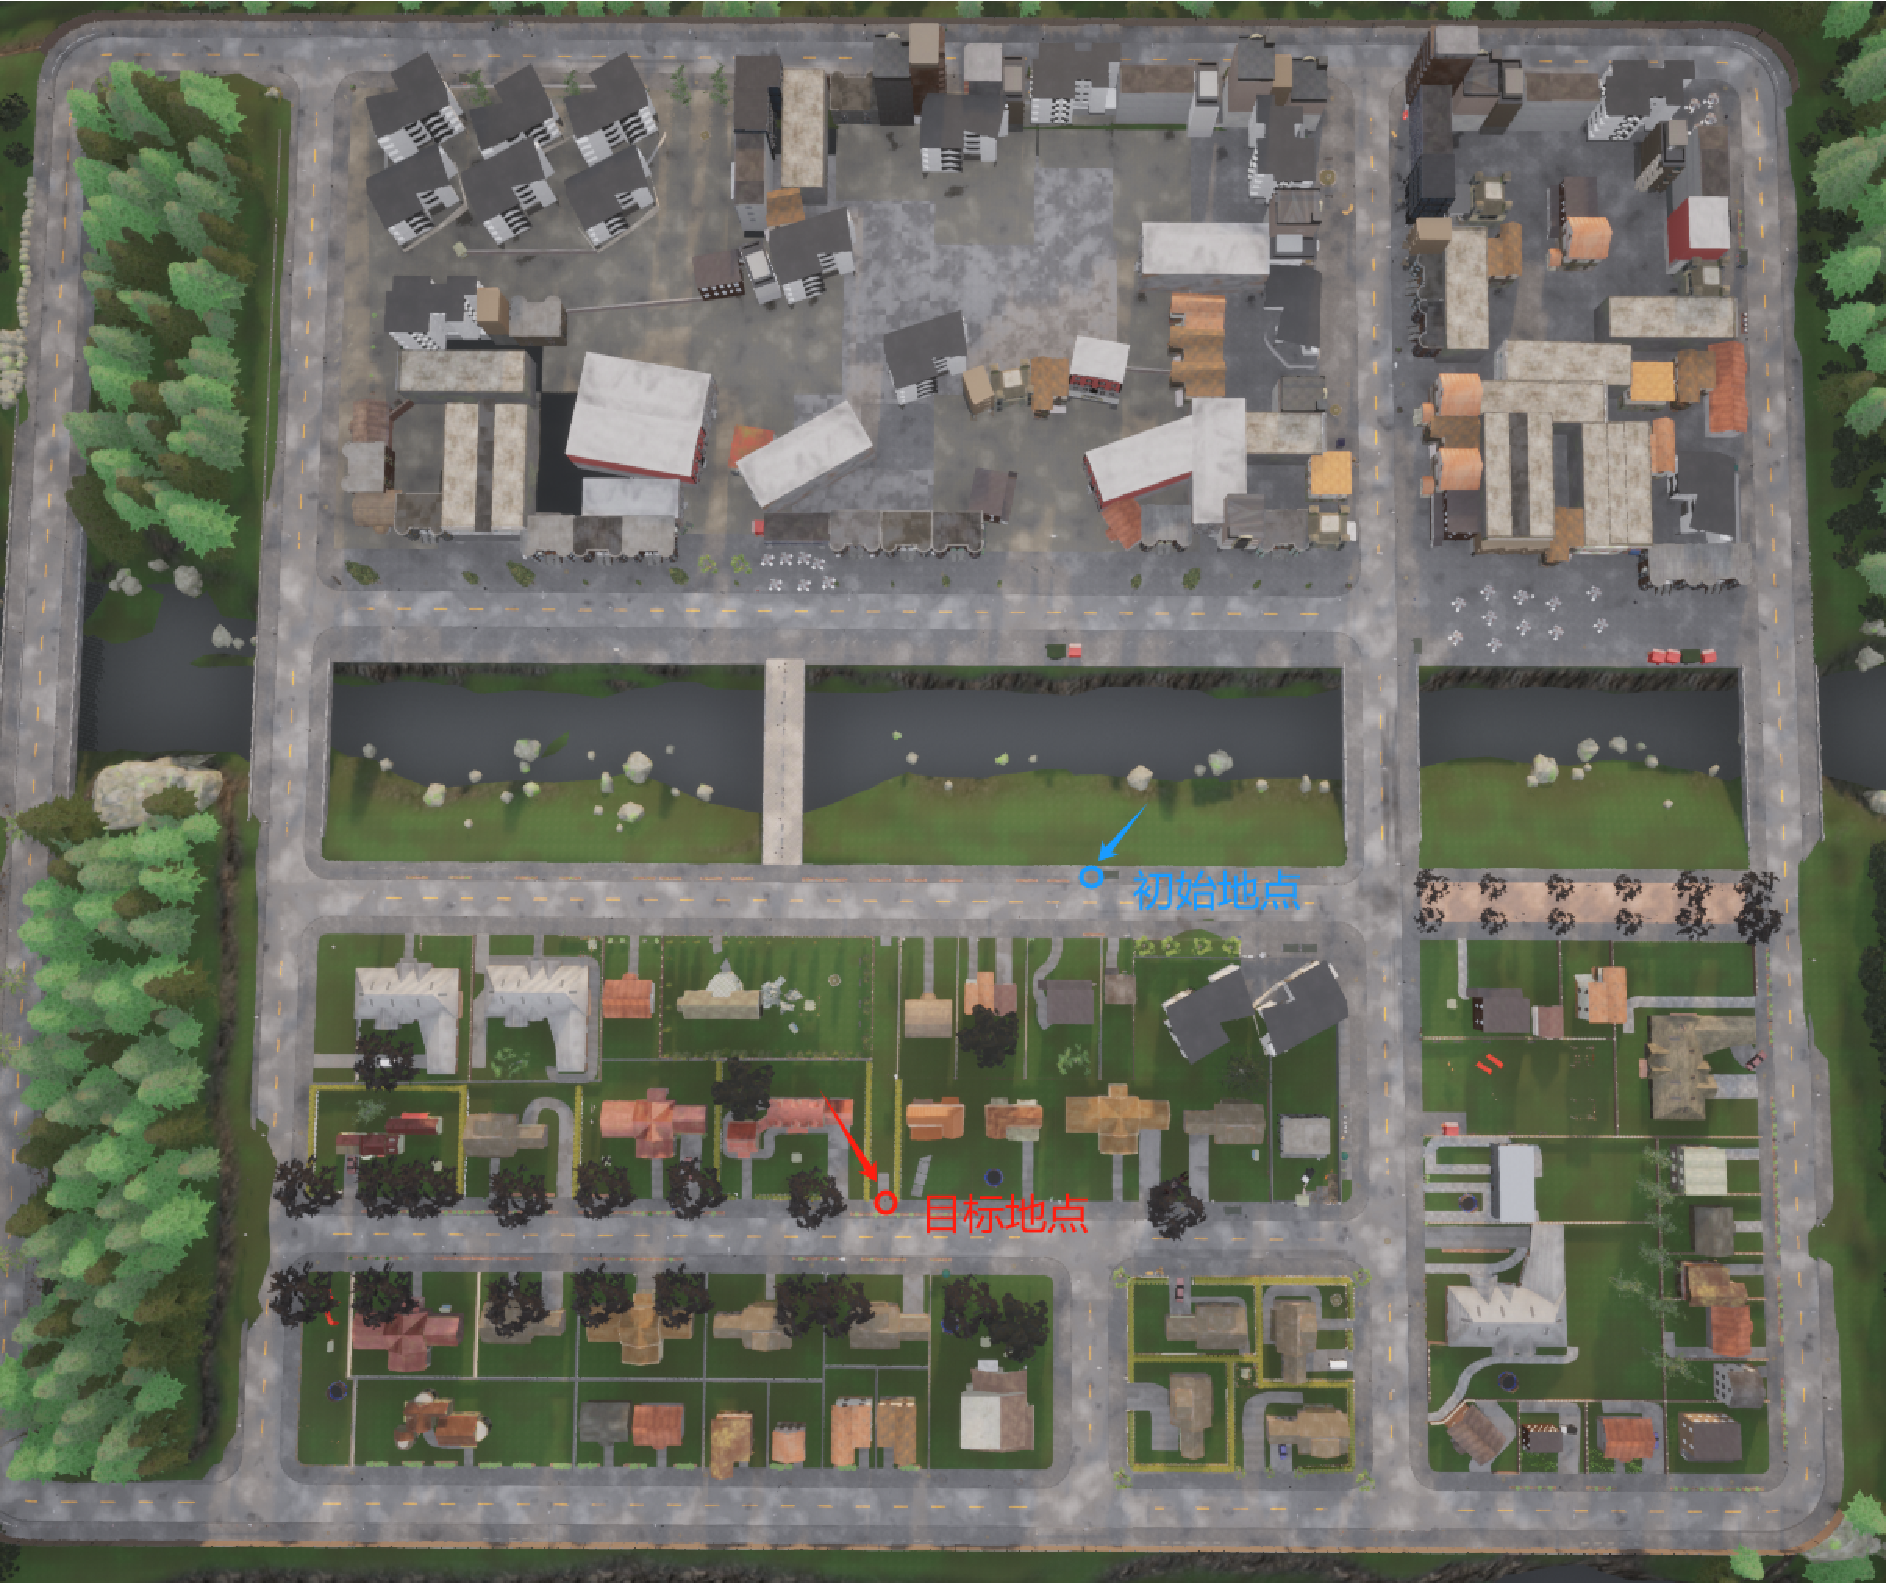
\includegraphics[width=0.8\textwidth]{images/location_select.pdf}
	    \caption{起始地点与目标地点示意图}
	    \label{fig:location}
	\end{figure}
	
	\section{奖励函数设计}
	
	强化学习任务中奖励函数设计至关重要,在行人导航系统中其直接影响智能体决策行为,合理设计奖励函数是实现高效稳定导航的关键,以下为本系统奖励函数的设计思想与实现细节:
	
	\subsection{目标达成奖励}
	目标达成奖励的目的是鼓励行人尽快接近目标,并在接近时给出更高的奖励。通过根据目标距离的变化量来调整奖励,确保模型能够学习到快速、有效的路径规划。
	
	\begin{equation}
	R_{\text{target}} =
	\begin{cases}
	1000 \cdot \mathbb{X}(d_{\text{target}}<3) & \text{终止条件} \\
	\Delta d \times 50 \times \left(1 - \frac{d_{\text{target}}}{100}\right) & \text{常规状态}
	\end{cases}
	\end{equation}
	其中:
	\begin{itemize}
	    \item \( \Delta d = d_{\text{prev}} - d_{\text{target}} \) 表示单步距离变化量
	    \item 动态系数强化近距离奖励:\( d_{\text{target}} \) 在 \([0, 100]\) 范围内时,系数从1.0线性衰减至0.0
	\end{itemize}
	
	\subsection{路径跟踪奖励}
	路径跟踪奖励旨在鼓励行人沿着预定的路径行进。通过计算行人与路径的横向偏差来调整奖励,确保行人尽量沿着正确的路线行走。
	
	\begin{equation}
	R_{\text{path}} =
	\begin{cases}
	1.5 \cdot \left(1 - \frac{\Delta_{\text{dev}}}{2}\right) & \Delta_{\text{dev}} \leq 2\ \text{m} \\
	-1.0 & \Delta_{\text{dev}} > 2\ \text{m}
	\end{cases}
	\end{equation}
	其中:
	\begin{itemize}
	    \item \( \Delta_{\text{dev}} = \left\| \vec{p}_{\text{current}} \times \vec{v}_{\text{forward}} \right\| / \left\| \vec{v}_{\text{forward}} \right\| \) 为路径偏差的计算方法
	\end{itemize}
	
	\subsection{安全避障机制}
	安全避障机制的目的是通过惩罚碰撞事件和危险距离来确保行人安全,避免与障碍物发生碰撞。
	
	\begin{equation}
	R_{\text{safety}} =
	\begin{cases}
	-500 \cdot \mathbb{X}_{\text{collision}} & \text{碰撞事件} \\
	-\dfrac{0.5}{d_{\text{obs}} + 0.5} & d_{\text{obs}} \leq 2\ \text{m} \\
	-(v_{\text{prev}} - v_{\text{curr}}) & \Delta v > 1\ \text{m/s}
	\end{cases}
	\end{equation}
	其中:
	\begin{itemize}
	    \item \( \mathbb{X}_{\text{collision}} \) 表示碰撞事件,碰撞时给予-500的惩罚。
	    \item \( d_{\text{obs}} \) 为障碍物的最小距离,若小于2米,则按距离反比例惩罚。
	    \item \( \Delta v = v_{\text{prev}} - v_{\text{curr}} \) 为速度变化,若速度骤降超过1米每秒,则给予惩罚。
	\end{itemize}
	
	\subsection{运动模式优化}
	运动模式优化的目的是确保行人的速度保持在合适范围内。通过设定不同速度区间的奖励,鼓励行人在不同距离的情境下选择合适的速度。
	
	\begin{equation}
	R_{\text{motion}} =
	\begin{cases}
	0.2 & \text{低速合规}(0.3 \leq v \leq 1.0)\ \cap\ d_{\text{target}} < 5\ \text{m} \\
	0.1 & \text{中速合规}(0.5 \leq v \leq 1.5) \\
	-0.2(v-1.0) & \text{超速状态}(v > 1.0)\ \cap\ d_{\text{target}} < 5\ \text{m}
	\end{cases}
	\end{equation}
	
	\subsection{时间效率惩罚}
	时间效率惩罚的目的是防止模型做出过多无效的移动或徘徊,鼓励快速完成任务。
	
	\begin{equation}
	R_{\text{time}} = -0.01 \cdot t_{\text{step}}
	\end{equation}
	其中:
	\begin{itemize}
	    \item 每一步都会施加一个固定的时间惩罚,以鼓励高效的路径规划。
	\end{itemize}
	
	\subsection{终止条件奖励}
	终止条件奖励的目的是当模型达到目标位置时给予额外奖励,或者在碰撞时进行终止。
	
	\begin{equation}
	R_{\text{terminal}} =
	\begin{cases}
	+1000 \cdot \mathbb{X}(d_{\text{target}} < 2\ \text{m}\ \cap\ \theta_{\text{error}} < 45^\circ) & \text{精确到达} \\
	-500 \cdot \mathbb{X}_{\text{collision}} & \text{碰撞终止}
	\end{cases}
	\end{equation}
	其中:
	\begin{itemize}
	    \item \( \theta_{\text{error}} = \left| \arctan\left(\frac{-\Delta y}{\Delta x}\right) - \theta_{\text{current}} \right| \) 表示当前朝向与目标方向之间的角度偏差。
	    \item 双重终止条件确保目标点朝向正确性。
	\end{itemize}
	
	\subsection{综合奖励架构}
	综合奖励架构的目的是将各个独立的奖励信号进行加权求和,形成一个最终的奖励值。这可以确保模型在考虑多个目标时进行平衡。
	
	\begin{equation}
	R_{\text{total}} = R_{\text{target}} + R_{\text{path}} + R_{\text{safety}} + R_{\text{motion}} + R_{\text{time}} + R_{\text{terminal}}
	\end{equation}
	其中:
	\begin{itemize}
	    \item \( R_{\text{target}} \) 为目标达成奖励
	    \item \( R_{\text{path}} \) 为路径跟踪奖励
	    \item \( R_{\text{safety}} \) 为安全奖励
	    \item \( R_{\text{motion}} \) 为运动模式奖励
	    \item \( R_{\text{time}} \) 为时间效率惩罚
	    \item \( R_{\text{terminal}} \) 为终止条件奖励
	\end{itemize}
	
	\subsection{具体实现}
	通过上述奖励函数的设计,行人导航系统能够有效地引导智能体在复杂环境中避开障碍物,迅速到达目标,并持续优化其决策策略,以实现最优路径规划。本节则描述了如何通过环境中的具体设置和传感器支持奖励的计算,实现导航。具体包括观测空间耦合、动态奖励系数、路径可视化等。
	
	\begin{itemize}
	    \item \textbf{观测空间耦合}:12维特征向量包含局部路径点坐标($x_{\text{wp}}, y_{\text{wp}}$)、障碍距离$d_{\text{obs}}$等。
	    \item \textbf{动态奖励系数}:目标距离因子$1 - \frac{d}{100}$实现奖励强度自适应。
	    \item \textbf{分层安全机制}:碰撞检测、障碍距离、速度变化三重防护。
	    \item \textbf{路径可视化}:通过Carla调试接口实时渲染路径点。
	\end{itemize}
	
	\section{路径规划与避障设计}
	
	路径规划与避障设计作为行人导航系统核心模块确保行人高效安全从起点抵达目标并避开动态环境障碍物,其实现依赖 Carla 仿真平台、强化学习(PPO 算法)及激光雷达(Lidar)和碰撞传感器等多种传感器输入。
	
	\subsection{路径规划}
	
	路径生成通过计算行人当前位置和目标位置之间的路径,利用Carla地图的get\_waypoint方法获取起点和终点的最近道路点,基于当前路径点选择下一个合适路径点,逐步生成从起点到终点的路径,路径点选择优先朝向目标位置的方向,直到路径接近目标,路径生成过程中进行平滑处理,减少路径突变,确保路径点之间平滑过渡。
	
	路径偏离检测实时更新路径偏离状态,计算行人当前位置和路径点之间的横向偏离,使用当前向量与前进方向的叉积确定偏离程度,若行人偏离预定路径,奖励机制会进行调整,鼓励行人保持在路径范围内。
	
	而路径规划部分通过计算起点到目标的最优路径,依赖行人当前状态、目标位置及环境障碍物信息,因需在动态环境中导航故需实时响应环境变化。强化学习训练时系统经反复试验学习最优路径选择,每一步依当前状态(含位置、朝向、速度、障碍物距离等)生成动作并据执行后的反馈学习,具体实施步骤为:根据行人当前状态计算与目标的方向和距离;使用 PPO 强化学习模型预测最佳动作(如直行、左转、右转等);动作执行后系统实时监测环境确保行人不偏离目标并避开障碍物。路径规划中奖励函数设计(如目标奖励)助力智能体持续优化路径选择以抵达目标。
	
	\subsection{避障设计}
	
	避障设计通过实时监控周围障碍物距离确保行人前进中有效避障防碰撞,本系统实现避障依赖的具体传感器和算法如下:激光雷达(Lidar)传感器实时检测障碍物距离和位置以判断是否避让并计算最小距离,碰撞传感器在碰撞时触发、记录事件并更新状态,避障算法通过计算行人与障碍物距离实时调整速度和方向,障碍物较近时减速或暂停以避免碰撞。避障功能与路径规划相互配合,系统检测到障碍物时避障算法自动调整行人路线避开障碍区域,障碍物避开后路径规划模块重新计算最优路径确保行人继续朝目标前进。
	
	在本系统中,避障功能与路径规划相互配合。当系统检测到障碍物时,避障算法会自动调整行人路线,避免进入障碍区域。一旦障碍物被避开,路径规划模块会重新计算最优路径,确保行人继续朝目标前进。
	
	\subsection{路径规划与避障的协同工作}
	
	路径规划与避障模块紧密配合以保障导航高效性和安全性,行人沿规划路径行进时系统通过激光雷达和碰撞传感器持续监控环境,检测到障碍物即执行避让操作,实时调整速度和方向避免碰撞,避障导致路径变化时路径规划模块即时重新计算最优路径并引导行人继续向目标行进,这种协同机制支持行人在复杂动态环境中稳定高效地完成导航任务。
	
	\section{优化设计}
	
	本行人导航系统对前有的PPO强化学习行人控制代码进行了优化,优化部分涵盖路径规划、避障策略控制及强化学习(PPO)模型优化。
	
	\subsection{路径规划控制}
	路径规划模块通过强化学习模型来选择最优路径。系统根据行人当前的状态(位置、速度、方向)以及目标位置,计算最佳路径。通过优化策略,系统逐步减少行人到目标的距离,并避免与障碍物发生碰撞。
	
	\subsection{避障控制}
	避障控制通过实时感知环境(激光雷达与碰撞传感器),确保行人能够避开障碍物。传感器提供周围障碍物的信息,避障模块基于这些信息调整行人的速度和方向。在强化学习的帮助下,系统可以在复杂的动态环境中快速做出避让决策。
	
	\subsection{强化学习优化}
	PPO算法在系统中的优化过程包括通过大量的训练来不断调整行人的行为策略。每次行进,系统会根据实际反馈(奖励函数)更新策略,以便更高效、更安全地完成任务。PPO算法能够处理高维状态空间,优化行人决策,使得行人在不断变化的环境中能够适应复杂的导航需求。
	
	\section{系统实现与测试}
	
	\subsection{系统实现}
	
	本行人导航系统基于 Carla 仿真平台并结合 PPO 强化学习算法实现路径规划与避障控制,主要模块如下:通过 Carla 客户端连接服务器并加载 “Town01” 地图,采用同步模式确保训练步骤中环境更新一致;利用 PPO 算法训练路径规划模型,依据当前状态预测最佳行进路径;借助激光雷达和碰撞传感器实时获取障碍物信息并调整路径以避免碰撞;通过 PPO 算法训练优化行人行为策略,提升行进效率与安全性。如图 \ref{fig:ped_nav},行人通过PPO算法导航即将到达目标地点,而目标地点使用的是Carla内置的障碍物Streetbarrier来作为可视化的标准。
	
	\begin{figure}[H]
	    \centering
	    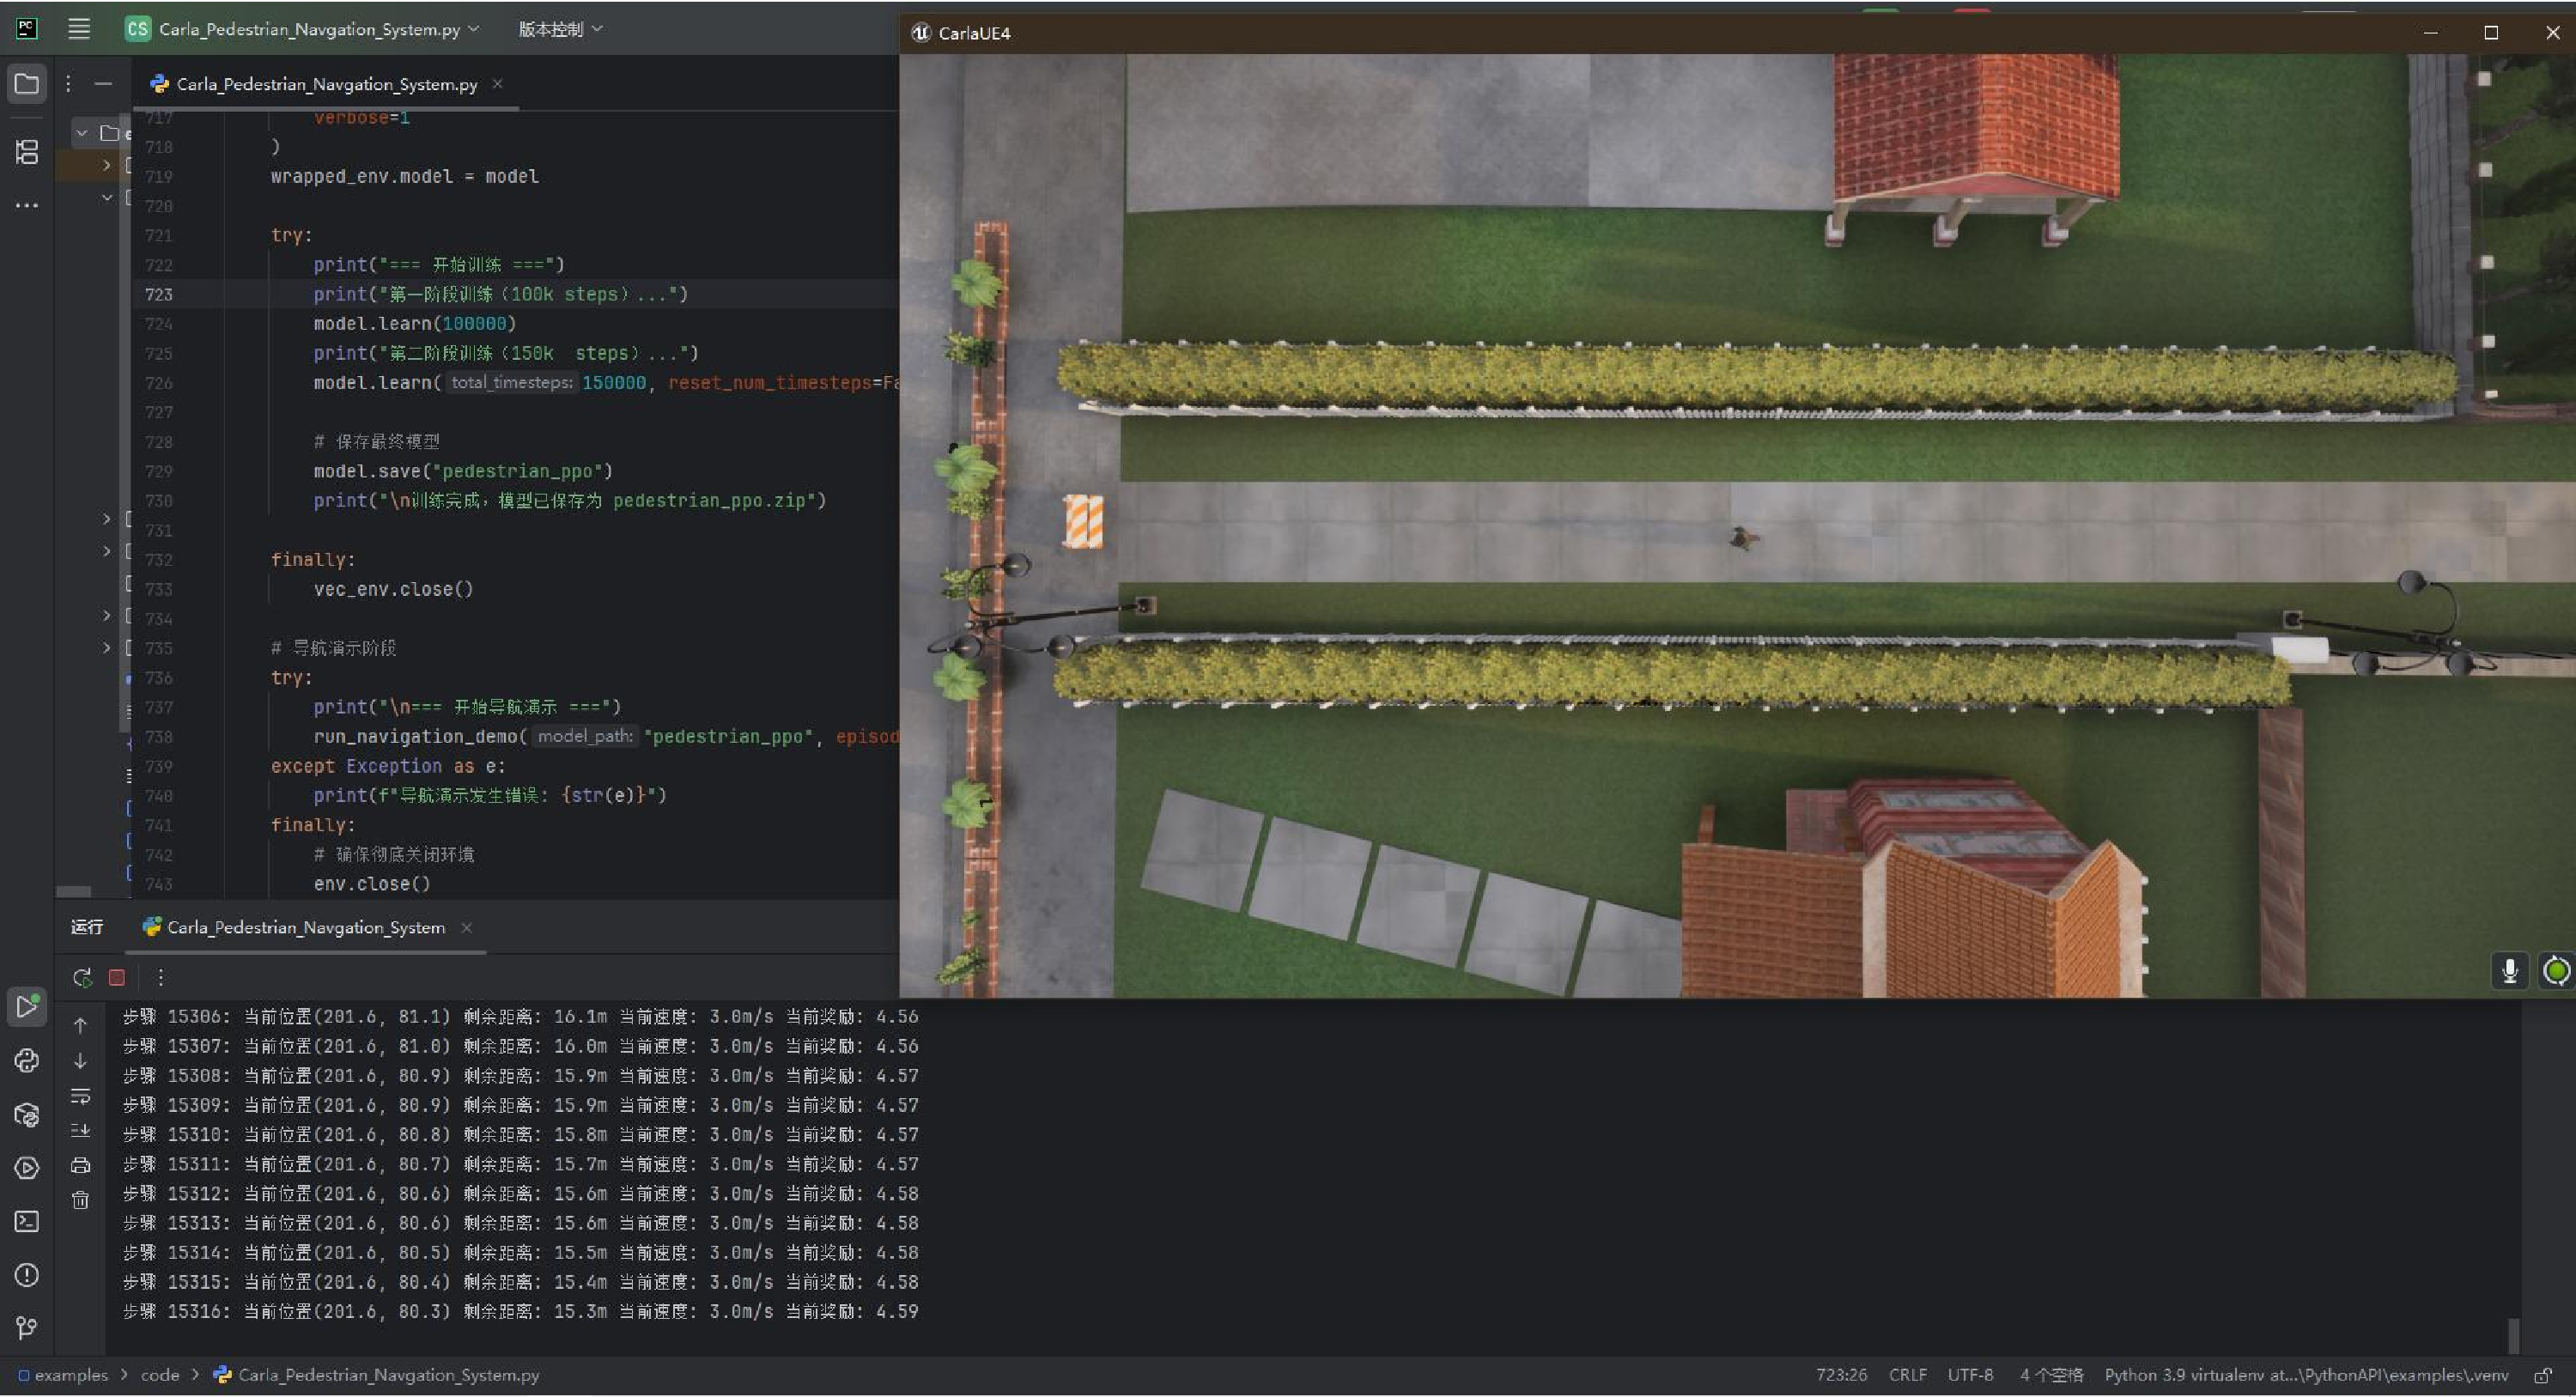
\includegraphics[width=0.8\textwidth]{images/pedestrain_navgation.pdf}
	    \caption{行人智能体通过PPO算法即将到达终点示意图}
	    \label{fig:ped_nav}
	\end{figure}
	
	\subsection{测试与验证}
	
	测试通过多次模拟训练与演示验证系统在复杂环境中的导航能力,主要测试目标涵盖:验证系统能否依据不同起点和终点实时计算最优路径;测试系统能否有效避开障碍物并保障行人安全;考察系统长时间运行稳定性尤其是在多障碍物动态环境中的表现。
